% !TeX spellcheck = cs_CZ
%---------------------------------------------------------------------------------------------------
% file spice.tex
%---------------------------------------------------------------------------------------------------
%================================= Kapitola: Osciloskopy a jejich použití ==========================
\setchaptertoc
\chapter{Osciloskopy a jejich použití}

  \section{Analogové osciloskopy}
  \section{Vzorkovací osciloskopy}
  \section{Digitální paměťové osciloskopy}
   

  \section{Pasivní sondy}

    \begin{figure}[ht!]
      \centering
      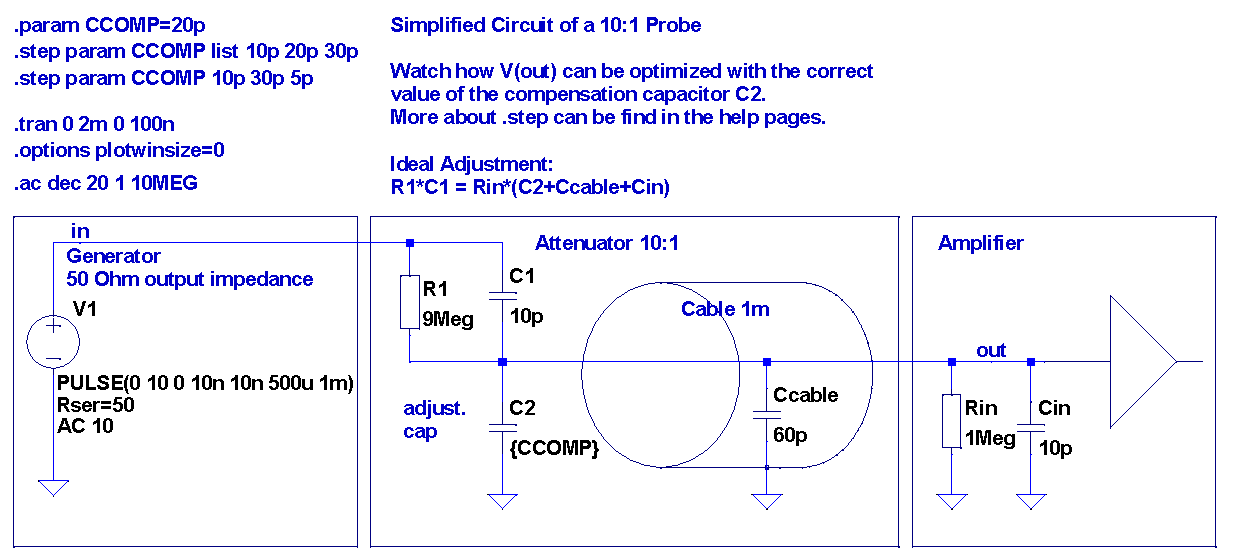
\includegraphics[width=1\linewidth]{../ltspice/ltc003_OSC_Probe_simple.pdf}
      \caption{\texttt{ltc002\_OSC\_Probe.asc}: }
      \label{SPICE:fig_ltc003_OSC}
    \end{figure}
    
    \begin{figure*}[ht!]
      \centering
      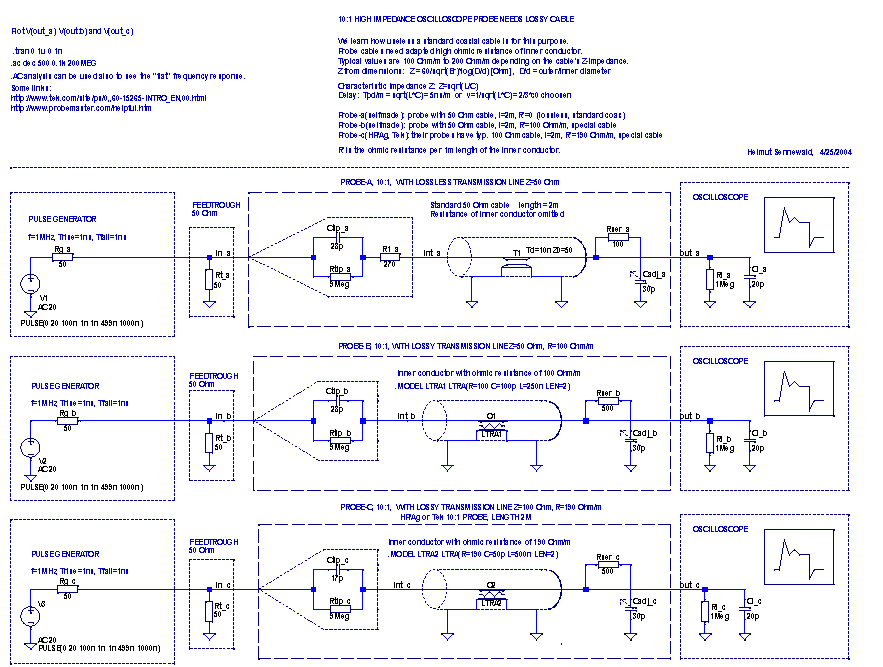
\includegraphics[width=1\linewidth]{../ltspice/ltc002_OSC_Probe.pdf}
      \caption{\texttt{ltc003\_OSC\_Probe\_simple.asc}: }
      \label{SPICE:fig_ltc002_OSC}
    \end{figure*}

  % \section{Aktivní sondy a proudové sondy}
  % \section{Stejnosměrná a střídavá vazba, odezva osciloskopu}
  % \section{Měření v koaxiálních obvodech}
  % \section{Časová refletometrie}
  % \section{Zobrazení XY}
  % \section{Kalibrace}
    

%---------------------------------------------------------------------------------------------------